\chapter{Конструкторская часть}
% В данном разделе сформулированы требования к разрабатываемому методу и разрабатываемому программному обеспечению. Разработан метод обнаружения фальсифицированного фрагмента на изображениях с использованием сверточной нейронной сети. Описаны основные этапы разработки в виде детализированной диаграммы IDEF0 и схема архитектуры разрабатываемой нейронной сети, а также изложены особенности предлагаемого метода. Спроектировано программное обеспечение для реализации разрабатываемого метода.
В этом разделе сформулируются требования к разрабатываемому методу и разрабатываемому программному обеспечению, описываются этапы работы алгоритма разрабатываемого метода, также рассматриваются структура разрабатываемой сверточной нейронной сети. Также описывается используемый набор данных для обучения модели и рассматривается структура программного обеспечения.

\section{Требования и ограничения к разрабатываемому методу}

К разрабатываемому методу предъявляются следующие требования.
\begin{itemize}[label = ---]
    \item Метод должен базироваться на использовании сверточных нейронных сетей с необходимыми модификациями.
    \item Принимать на вход изображения в форматах PNG, JPG, JPEG, BMP с размером от $216 \times 216$ до $1024 \times 1024$ включительно.
    \item Метод должен быть применим для работы с различными типами сцен, а также различными освещением.
\end{itemize}

К разрабатываемому программному обеспечению предъявляются следующие требования.
\begin{itemize}[label = ---]
    \item Возможность загрузки изображений в формате PNG, JPG, JPEG или BMP.
    \item Возможность обработки как RGB~--~изображений.
    \item Возможность просмотра информации по процессу обучения модели.
    \item Возможность просмотра значения метрик качества модели.
    \item Разрабатываемое ПО должно корректно реагировать на любые действия пользователя.
\end{itemize}
% \newpage
\section{Описание разрабатываемого метода}

\subsection{Декомпозиция разрабатываемого метода}
Ниже, на рисунке \ref{img:idef0-1}, представлена IDEF0-диаграмма разрабатываемого метода первого уровня.

\captionsetup{justification=centering,singlelinecheck=off}
\begin{figure}[h!]
	\centering
		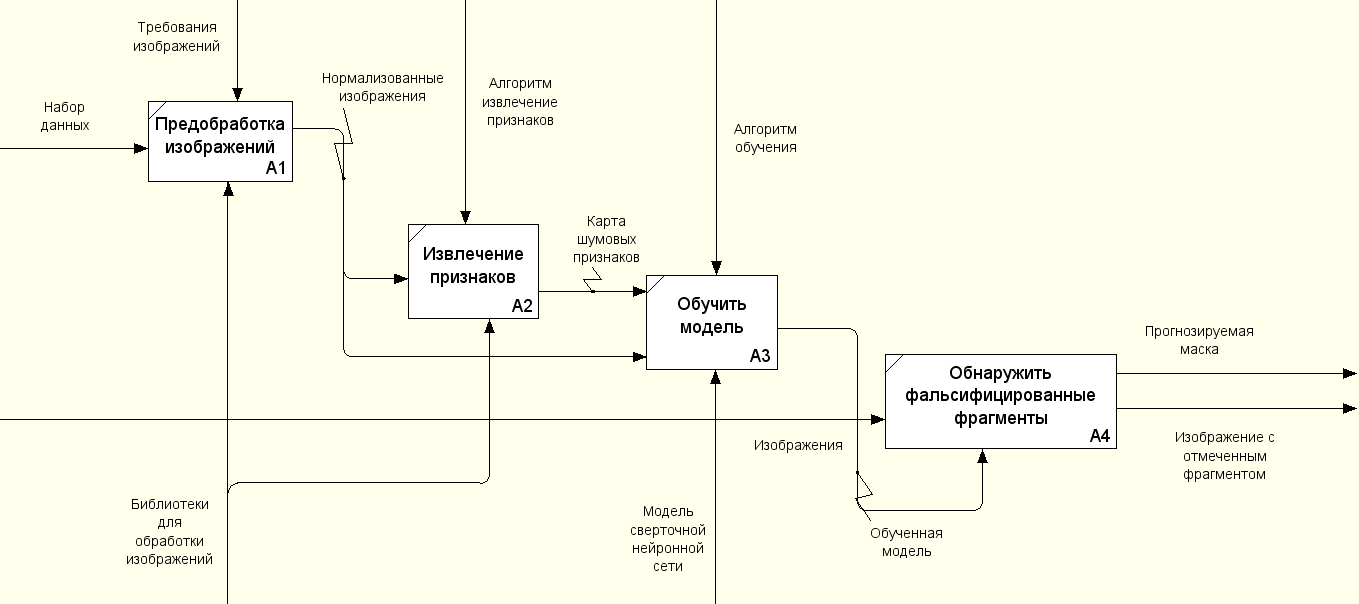
\includegraphics[,scale=0.45]{./img/idef0-1.png}
		\caption{IDEF0-диаграмма первого уровня}  
		\label{img:idef0-1}
\end{figure}

Разрабатываемый метод обнаружения фальсифицированного фрагмента на изображении состоит из четырёх последовательных этапов. Первый этап — предобработка, которая включает нормализацию входного изображения, приведение его к единому размеру и подготовку данных для последующего анализа. Второй этап — извлечение признаков — заключается в формировании карты шумовых признаков.  Данный этап критически важен, поскольку именно шумовая карта несёт в себе следы неоднородности, возникающие при вставке фрагмента из другого изображения или при повторном сжатии. Алгоритм извлечения признаков спроектирован так, чтобы подчеркнуть высокочастотные составляющие, в которых маскируются артефакты фальсификации. Третий этап — обучение модели — представляет собой процесс настройки параметров двухпоточной свёрточной нейронной сети с использованием подготовленного размеченного набора данных, включая оптимизацию весов, слоёв адаптации признаков и механизмов внимания. Четвёртый этап — обнаружение фальсификации — заключается в применении обученной модели к новым изображениям для получения пиксельной маски локализации подделанного фрагмента. Такая декомпозиция позволяет чётко разделить функциональные обязанности между модулями программного обеспечения и обеспечивает гибкость.

\subsection{Алгоритмы предобработки и извлечения признаков}
Основная цель предварительной обработки изображений перед их подачей в сверточную нейронную сеть (CNN) — повысить качество и информативность данных, чтобы улучшить детектирование артефактов, характерных для глубогого подделки. Этот этап помогает устранить шумы, нормализовать изображения, выделить ключевые признаки и минимизировать влияние вариаций освещения, масштаба и ракурса. В результате CNN может более эффективно фокусироваться на различиях между реальными и синтетическими изображениями, повышая точность обнаружения \cite{preprocessing1}.

Кроме того, предобработка включает в себя приведение всех изображений к единому цветовому пространству RGB и масштабирование интенсивности пикселей к диапазону [0,1], что стандартизирует входной сигнал для нейронной сети. Без такой нормализации градиенты могут стать нестабильными, а процесс обучения — замедлиться.
Ниже, на рисунке \ref{img:preprocessing}, преставлены шаги предобработка изображения.
\captionsetup{justification=centering,singlelinecheck=off}
\begin{figure}[h!]
	\centering
		
\includegraphics[,scale=0.9]{./img/preprocessing.png}
		\caption{Шаги предобработка изображения}  
		\label{img:preprocessing}
\end{figure}
\newpage
Для извлечения признаков из изображений используются карты щумовыых признаков. 

Ниже на рисунку \ref{img:algorithm} показан алгоритм извлечения карты щумовыых признаков.

\captionsetup{justification=centering,singlelinecheck=off}
\begin{figure}[h!]
	\centering
		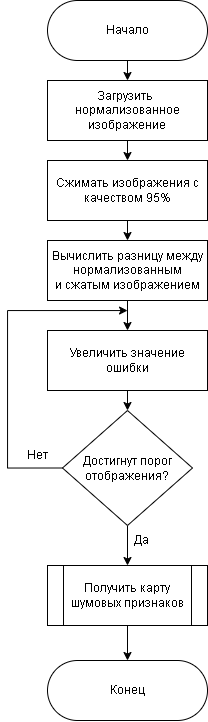
\includegraphics[,scale=0.8]{./img/algo.png}
		\caption{Алгоритм извлечения признаков.}  
		\label{img:algorithm}
\end{figure}
% \newpage

После завершения предварительной обработки запускается итеративный алгоритм выделения шумовых признаков. На вход подаётся нормализованное изображение. Оно сжимается с качеством 95\% — это создаёт потери, характерные для сжатия. Затем вычисляется попиксельная разность между исходным нормализованным изображением и его сжатой версией. Полученная разность усиливается — значение ошибки увеличивается. После усиления проверяется, достигнут ли заданный порог отображения. Если порог не достигнут, цикл повторяется: снова вычисляется разность. Как только порог оказывается превышен, алгоритм формирует итоговую карту шумовых признаков. Таким образом, метод многократно накапливает и усиливает малые искажения, обусловленные сжатием, что позволяет выделить слабые артефакты, которые в дальнейшем могут служить характерными признаками для обнаружения.

Эта предобработка позволяет CNN сосредоточиться на анализе наиболее значимых для обнаружения подделок областей, повышая точность модели.

\subsection{Структура разрабатываемой сверточной нейронной сети}

Разрабатываемая сверточная нейронная сеть представляет собой многоуровневую архитектуру, специально спроектированную для эффективного извлечения признаков из изображений. Модель сочетает в себе последовательную обработку через блоки свёртки, cлои адаптации признаков и механизмы внимания.

Выбор двухпоточной архитектуры обусловлен необходимостью разделить анализ низкоуровневых шумовых артефактов и высокоуровневого семантического содержания. Шумовой поток оперирует картой остаточных ошибок, которая чувствительна к манипуляциям, но бедна по семантике, тогда как RGB-поток сохраняет информацию о форме, цвете и текстуре объектов. Слияние этих двух потоков в глубоких слоях сети позволяет модели выявлять несоответствия, например, когда семантически корректный объект имеет неправильную шумовую характеристику.

Общая структура сети показана на рисунке \ref{img:cnn-architecture}.

\captionsetup{justification=centering,singlelinecheck=off}
\begin{figure}[h!]
	\centering
		
\includegraphics[,scale=0.6]{./img/cnn.png}
		\caption{Общая структура сети.}  
		\label{img:cnn-architecture}
\end{figure}

Cтруктура сети делится на две основные ветви, работающие с разными представлениями входных данных. Первая ветвь обрабатывает карту шумовых признаков изображения, полученную предварительно. Вторая ветвь работает непосредственно с нормализованным исходным изображением. Такое двухпотоковое проектирование позволяет сети одновременно учитывать как низкоуровневые шумовые артефакты, так и высокоуровневые семантические особенности изображения. Cтруктура сети включает три ключевых типа компонентов: блоки свёртки, слои адаптации признаков и слои внимания, которые работают в тесной взаимосвязи.

Блок свёртки является базовым строительным элементом сети. Каждый такой блок представляет собой последовательность операций, типичную для современных CNN: свёртку 3×3, нормализацию пакетную и функцию активации ReLU. 

Ниже, на листинге \ref{code:conv}, показана реализация блока свёртки.

\begin{lstlisting}[caption=Листинг 2.1 -- Реализация блока свёртки,label=code:conv]
	self.conv1 = nn.Sequential(
		nn.Conv2d(3, bn, kernel_size=3, padding=1),
		nn.BatchNorm2d(bn),
		nn.ReLU(True)
	)
\end{lstlisting}

Блоки свёртки отвечают за извлечение иерархических признаков на разных масштабах. Благодаря использованию свёрток с размером ядра 3×3 и дополнением сохраняется пространственное разрешение карт признаков, что важно для последующей точной локализации границ подделки. Нормализация пакетов ускоряет обучение и стабилизирует динамику градиентов, а нелинейность ReLU вносит необходимую нелинейность, позволяя сети аппроксимировать сложные функции.

Понижение разрешения выполняется не с помощью стандартных операций пулинга (например, MaxPooling или AveragePooling), а с помощью свёрточных слоёв с шагом больше 1. Это позволяет не только уменьшить пространственные размеры карт признаков, но и одновременно увеличить глубину каналов, а также изучить более информативные признаки, так как свёртка с шагом является обучаемой операцией.

На листинге \ref{code:downsampling} показана реализация слоя уменьшения разрешения.

\begin{lstlisting}[caption=Листинг 2.2 -- Реализация слоя уменьшения разрешения,label=code:downsampling]
	self.conv1b = nn.Sequential(
    nn.Conv2d(bn, bn, kernel_size=4, padding=1, stride=2),
    nn.BatchNorm2d(bn),
    nn.ReLU(True)
)
\end{lstlisting}

Здесь ядро свёртки имеет размер 4×4, шаг 2 и дополнение 1, что приводит к уменьшению высоты и ширины карты признаков в два раза. Такой подход обеспечивает лучшее сохранение информации по сравнению с пулингом и способствует формированию инвариантных к мелким смещениям признаков.

В модели используются несколько последовательных блоков downsampling, что позволяет построить пирамиду признаков с различными масштабами (от полного разрешения до 1/8, 1/16 и т.д.). Это необходимо для захвата как мелких деталей, так и глобального контекста.

Для восстановления пространственного разрешения до размера входного изображения применяется билинейная интерполяция с последующей свёрткой 1×1 для согласования числа каналов. Такой подход широко используется в энкодер-декодер архитектурах, так как он прост в реализации и не вносит дополнительных обучаемых параметров.

На листинге \ref{code:upsampling} показана реализация слоя увеличения разрешения.

\begin{lstlisting}[caption=Листинг 2.3 -- Реализация слоя увеличения разрешения,label=code:upsampling]
	self.deconv4 = nn.Sequential(
	nn.Upsample(scale_factor=2, mode='bilinear', align_corners=True),
	nn.Conv2d(bn*4, bn*4, kernel_size=1))
\end{lstlisting}

Сначала с помощью nn.Upsample увеличивается размер карты признаков до нужной высоты и ширины (bw, bh), затем свёртка 1×1 изменяет количество каналов. После этого часто следуют дополнительные свёрточные слои (3×3), нормализация и активация, которые позволяют уточнить восстановленные признаки.

В модели слой увеличения размерности выполняется на нескольких уровнях, при этом результаты объединяются со остаточными связями с соответствующими картами признаков из энкодерной части. Это позволяет эффективно восстанавливать пространственные детали, которые могли быть потеряны при уменьшения размерности.

Слои адаптации признаков — это специализированные модули, которые обеспечивают эффективное согласование и слияние признаков, поступающих из двух параллельных потоков (шумового и RGB-потока). Каждый такой слой принимает на вход карту признаков из соответствующего потока и применяет к ней ряд преобразований: 1×1-свёртку для изменения количества каналов, остаточное соединения и нормализацию. 

Ниже на рисунке \ref{img:fal} представлена структура слоя адаптации признаков.

\captionsetup{justification=centering,singlelinecheck=off}
\begin{figure}[h!]
	\centering
		
\includegraphics[,scale=1.15]{./img/fal.png}
		\caption{Слой адаптации признаков.}  
		\label{img:fal}
\end{figure}

Основная задача этих слоёв — привести признаки из разнородных доменов (шум и естественное изображение) к единому представлению, минимизируя доменное расхождение и усиливая полезные для задачи обнаружения фальсифицированного фрагмента. 

Ниже, на листинге \ref{code:fal}, показана реализация слоя адаптации признаков.

\begin{lstlisting}[caption=Листинг 2.4 -- Реализация слоя адаптации признаков,label=code:fal]
	DL4 = self.deconv4(L52)
	DL4_add = DL4 + L4   

	DL44 = self.deconv44(L55)
	DL44_add = DL44 + L44   
	DL44b = self.deconv44b(DL44_add)
	DL44bada = DL44b + DL44_add 

	DL4_cat = torch.cat([DL4_add, L4c, DL44bada], 1)

	DL4_att = self.att4(DL4_cat)
	DL4b = self.deconv4b(DL4_att)
\end{lstlisting}

Слои адаптации признаков спроектированы как остаточные блоки (англ. residual blocks) с операциями свёртки 1×1, нормализации и сложения с исходным тензором. Такая архитектура выбрана для согласования признаков, поступающих из двух различных доменов – шумовой карты и RGB-изображения. Поскольку эти два потока имеют существенно разные статистические распределения (высокочастотный шум против семантически насыщенных цветовых текстур), прямое объединение их карт признаков приводит к сильным помехам и размытию границ предсказанной маски. Остаточные блоки позволяют эффективно фильтровать помехи, сохраняя при этом полезную высокочастотную информацию за счёт skip-соединений, которые обеспечивают передачу исходных признаков на выход блока. Это объясняется тем, что остаточные соединения облегчают обучение, позволяя градиентам беспрепятственно проходить через слой, а также дают возможность сети «довычитывать» невязку между разнородными представлениями, что ведёт к более точной локализации даже на сложных текстурах. Таким образом, выбор остаточной архитектуры для адаптации признаков является оптимальным компромиссом между сохранением дискриминативной информации и подавлением междоменных шумов, что подтверждается полученными количественными показателями.

Слои внимания являются важнейшим механизмом выделения релевантных признаков сети. Эти слои динамически перевешивают важность различных каналов и пространственных областей, позволяя сети концентрироваться на областях с высокой вероятностью манипуляции. Особенно эффективно слои внимания работают после слияния двух потоков, помогая выделить несоответствия между шумовыми аномалиями и семантическим содержимым. Слой внимания включает глобальный пулинг, два полносвязных слоя с активациями ReLU и Sigmoid, а также операцию масштабирования, что позволяет динамически перераспределять веса по каналам карты признаков. Их структура представлена ниже, на рисунке \ref{img:seam}.

\captionsetup{justification=centering,singlelinecheck=off}
\begin{figure}[h!]
	\centering
		
\includegraphics[,scale=1.1]{./img/seam.png}
		\caption{Слой внимания.}  
		\label{img:seam}
\end{figure}

% \newpage

Слой внимания работает следующим образом: сначала глобальный усредняющий пулинг сжимает пространственную размерность карты признаков, формируя вектор описания каналов. Затем два полносвязных слоя (с уменьшением размерности и последующим восстановлением) вычисляют веса важности для каждого канала. После применения сигмоидной функции эти веса нормализованы в диапазоне [0,1] и умножаются на исходную карту признаков, усиливая значимые каналы и подавляя неинформативные. Такой механизм особенно полезен для обнаружения фальсификаций, так как поддельные области часто активируют лишь небольшое подмножество каналов.

Слой внимания построен по принципу сжатия-возбуждения (англ. Squeeze-and-Excitation, SE), который позволяет динамически перекалибровывать канальные веса карт признаков. Такая архитектура выбрана потому, что при обнаружении фальсифицированных фрагментов решающую роль играют не все каналы одинаково: высокочастотные шумовые артефакты, характерные для подделок, сосредоточены в определённых каналах, тогда как большинство каналов несут информацию о подлинном фоне. Механизм SE, состоящий из глобального усредняющего пулинга, двух полносвязных слоёв с нелинейностями ReLU и Sigmoid, позволяет сети научиться выделять именно те каналы, которые содержат дискриминативные признаки манипуляции. Это особенно важно при сильном дисбалансе классов, когда область подделки занимает менее 5–10 \% площади изображения. Таким образом, выбор именно такой структуры внимания обусловлен её способностью фокусироваться на релевантных артефактах и подавлять фоновый шум, что критически важно для точной локализации границ фальсификации.

На листинге \ref{code:seam}, показана реализация слоя внимания.

\begin{lstlisting}[caption=Листинг 2.5 -- Реализация слоя внимания,label=code:seam]
	class SELayer(nn.Module):
    def __init__(self, channel, reduction=16):
        super(SELayer, self).__init__()
        self.avg_pool = nn.AdaptiveAvgPool2d(1)         
        self.fc = nn.Sequential(
            nn.Linear(channel, channel // reduction, bias=False),
            nn.ReLU(inplace=True),
            nn.Linear(channel // reduction, channel, bias=False),
            nn.Sigmoid()                                 
        )

    def forward(self, x):
        b, c, _, _ = x.size()
        y = self.avg_pool(x).view(b, c)                  
        y = self.fc(y).view(b, c, 1, 1)                  
        return x * y.expand_as(x)    
\end{lstlisting}

Общая структура сети организована по принципу двух параллельных ветвей с последующим многоуровневым слиянием и декодером. Входные данные поступают в сеть по двум независимым путям. Верхний поток начинается с карты шумовых признаков, полученной предварительно. Этот поток использует блоки свёртки и слои уменьшения размерности, постепенно извлекая характерные шумовые паттерны, возникающие при JPEG-сжатии, копировании-вставке и так далее. На нескольких уровнях глубины из этого потока ответвляются признаки в слои адаптации признаков, где они приводятся в соответствие с признаками из второго потока.

Нижний поток принимает нормализованное RGB-изображение. Он также состоит из последовательности блоков свёртки и downsampling-слоёв, но сохраняет больше информации о цветовом и текстурном содержимом. После нескольких стадий извлечения признаков происходит поэтапное слияние информации из обоих потоков через слои адаптации признаков.
После слияния на нескольких масштабах объединённые признаки проходят через последовательность слоёв внимания, которые уточняют представление, подавляя шум и усиливая области с подозрительными артефактами. Далее следует декодирующая часть сети, включающая слои увеличения размерности, skip-соединения с ранними уровнями энкодера и финальные свёрточные блоки. Завершается архитектура выходным слоем, формирующим карту локализации подделки с тем же пространственным разрешением, что и исходное изображение.

Использование пропущенных связей между энкодером и декодером позволяет восстанавливать мелкие пространственные детали, которые иначе теряются при многократном уменьшении разрешения. Это критически важно для точного определения границ фальсифицированного фрагмента, особенно если он имеет небольшие размеры или сложную форму. В предложенной сети пропущенные связи организованы на четырёх масштабных уровнях, что обеспечивает высокую точность сегментации.

Такое сочетание двухпоточной обработки, модулей адаптации признаков и механизмов внимания позволяет сети эффективно обнаруживать как локальные, так и глобальные манипуляции, сохраняя при этом хорошую обобщающую способность на различных типах подделок и различных источниках изображений. Архитектура является достаточно лёгкой для обучения на современных графического процессора, но при этом обладает высокой выразительной силой благодаря продуманному взаимодействию между шумовым и визуальным доменами.
В целом, предложенная структура разрабатываемой сверточной нейронной сети сочетает в себе классические принципы CNN  с современными механизмами, что делает её особенно подходящей для сложной и практически значимой задачи обнаружения цифровых фальсификации изображений.

\section{Структура разрабатываемого программного обеспечения}

Разрабатываемое программное обеспечение состоит из двух модулей:
\begin{itemize}[label=---]
    \item модуль, реализующий метод обнаружения фальсифицированного фрагмента на изображениях с использованием сверточной нейронной сети;
    \item пользовательское приложение, производящее обнаружение фальсифицированного фрагмента на изображениях на основе разработанного метода, а так же предоставляющее возможность обучения модели, используемой в предыдущем модуле.
\end{itemize}
\subsection*{Модуль CNN модели}
В данном модуле происходит только обучение и сохранение модели. Модуль должен быть использован либо при первоначальном обучении модели.

Входными данными для модуля является набор данных CASIA v2.0, содержащий пары «исходное изображение – бинарная маска разметки». Результатом работы модуля является файл, содержит в себе обученную модель, т.е. ее структуру и весовые коэффициенты соответствующих связей. Это необходимо для того, чтобы не тратить время на обучение модели при повторном использовании, так как процесс обучения может занимать продолжительный период времени в зависисмотси от некоторых факторов.

На рисунке~\ref{img:module-cnn} представлена схема работы с модулем CNN модели.
\begin{figure}[h!]
	\centering
		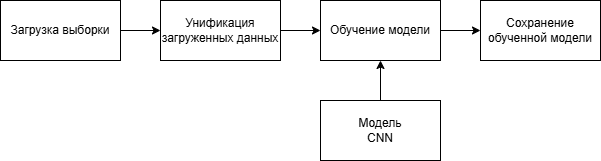
\includegraphics[,scale=0.8]{./img/model1.png}
		\caption{Схема работы с модулем CNN модели}  
		\label{img:module-cnn}
\end{figure}
\subsection*{Модуль пользовательского приложения}

Данный модуль реализует непосредственное обнаружение фальсифицированных фрагментов на изображениях, загружаемых пользователем. Входными данными для модуля является цветное изображение в одном из поддерживаемых форматов (PNG, JPG, JPEG, BMP, TIF), а также заранее обученная модель, сохранённая на предыдущем этапе. Модуль формирует выходные данные: исходное изображение с наложенными полупрозрачными ограничивающими рамками и тепловой картой, а также отдельно бинарную маску подделки. Вся эта информация отображается в пользовательском интерфейсе вместе со служебными данными — процентом и количеством фальсифицированных пикселей и временем обработки. Пользователь может скопировать полученный отчёт или сохранить результат в виде изображения. Таким образом, модуль приложения обеспечивает полный цикл анализа, от загрузки изображения до визуализации и предоставления количественных результатов, делая систему доступной для конечного пользователя.

На рисунке~\ref{img:module-user} представлена схема работы с модулем пользовательского приложения.

\begin{figure}[h!]
	\centering
		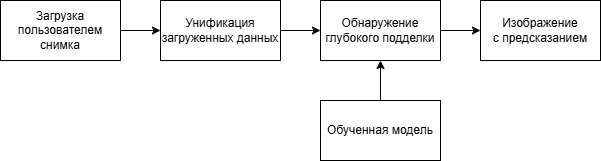
\includegraphics[,scale=0.75]{./img/module-user.png}
		\caption{Схема работы с модулем пользовательского приложения}  
		\label{img:module-user}
\end{figure}
% \newpage
\section{Набор данных для обучения модели}
Для обучения и оценки модели использовался широко известный в области цифровой криминалистики набор данных CASIA v2.0. Данный датасет был считается одним из наиболее крупных и сложных публичных наборов данных для задач обнаружения и локализации различных типов манипуляций с изображениями\cite{casia1}.

CASIA v2.0 содержит 5123 поддельных изображений и соответственные бинарные маски. Поддельные изображения включают два основных типа манипуляций: copy-move (копирование и вставка внутри одного изображения) и splicing (вставка объектов из других изображений). Изображения имеют различное разрешение и представлены в нескольких форматах: PNG, JPEG и TIFF. Важной особенностью датасета является наличие постобработки поддельных областей (размытие, сжатие, поворот, масштабирование), что делает задачу локализации значительно более сложной и приближенной к реальным условиям.

Применение CASIA v2.0 позволило модели обучаться на разнообразных сценариях подделок, различных текстурах, освещении и постобработках, что существенно повышает обобщающую способность сети. Перед обучением изображения проходили этап нормализации и предварительной аугментации для повышения устойчивости модели к вариациям условий съёмки и сжатия.

Использование именно этого датасета обеспечивает возможность объективного сравнения результатов предлагаемой модели с существующими современными подходами в области обнаружения цифровой фальсификации изображений.

Ниже, на рисунке~\ref{img:casia} представлен пример изображений из набора данных CASIA v2.0.

\captionsetup{justification=centering,singlelinecheck=off}
\begin{figure}[h!]
	\centering
		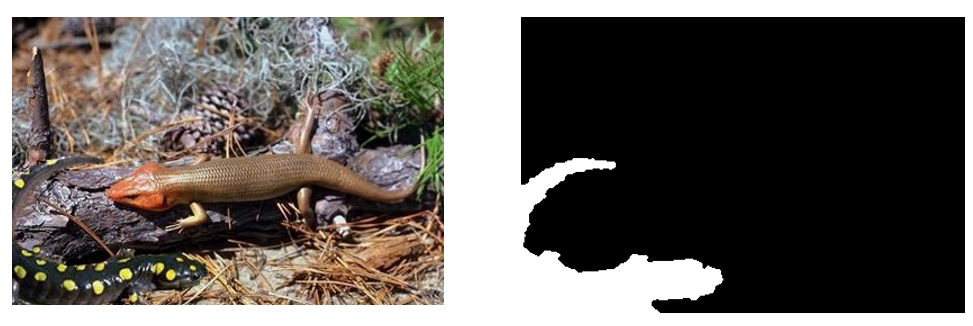
\includegraphics[,scale=0.6]{./img/casia.png}
		\caption{Пример изображений из набора данных CASIA v2.0}  
		\label{img:casia}
\end{figure}

\section*{Вывод}
\addcontentsline{toc}{section}{Вывод}

В этом разделе были сформулированы требования к разрабатываемому методу и разрабатываемому программному обеспечению и описаны этапы работы алгоритма разрабатываемого метода, также была рассматривана структура разрабатываемой сверточной нейронной сети. Был описан используемый набор данных для обучения модели и была рассмотрена структура программного обеспечения.